%\usepackage[T1]{fontenc}
%\usepackage[utf8]{inputenc}

%!TEX ROOT=../diploma-thesis.tex

\chapter{Návrh}\label{ch:navrh}

V této kapitole ...

\section{Formalizace architektury orientované na služby}

\subsection{Join-points}

\begin{figure}
    \centering
    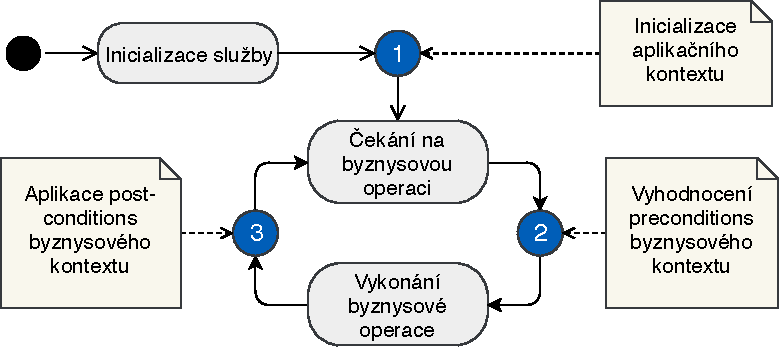
\includegraphics[keepaspectratio=true, width=0.8\linewidth]{figures/join-points.pdf}
    \caption{Diagram životn\'{\i}ho cyklu služby a identifikovan\'ych join-pointů}
    \label{fig:join-points}
\end{figure} % TODO: popsat

\subsection{Advices}

\subsection{Pointcuts}

\subsection{Weaving}

\section{Architektura frameworku}

\section{Zachycen\'{\i} byznysového konextu}

Př\'{\i}stup \gls{ADDA} doporučuje popsat byznysová pravidla pomoc\'{\i}
vlastn\'{\i}ho, na m\'{\i}ru šitého, doménově specifického jazyka~\cite{cemus2015automated}.
V našem př\'{\i}padě můžeme jazykem \gls{DSL} popsat kompletně i cel\'y
byznysov\'y kontext.

V sekci~\ref{sec:business-rule-dls} jsme zjistili, že ačkoliv jsou nástroje Drools a JetBrains
MPS velmi silnými aparáty, jejich vlastnosti nejsou plně vhodné pro řešení problému
centrální administrace a automatické distribuce byznysových pravidel.
Můžeme jít cestou volby co nejvhodnějšího jazyka pro každou platformu, kterou chceme
využívat pro naše účely, a implementace adapterů pro tyto jazyky, které transformují
dané \gls{DSL} do reprezentace vhodné pro využití naším frameworkem. Vzhledem k
různým vlastnostem těchto jazyků by takový přístup byl suboptimální.

\section{Metamodel byznys kontextu}\label{sec:metamodel}

\begin{figure}
    \centering
    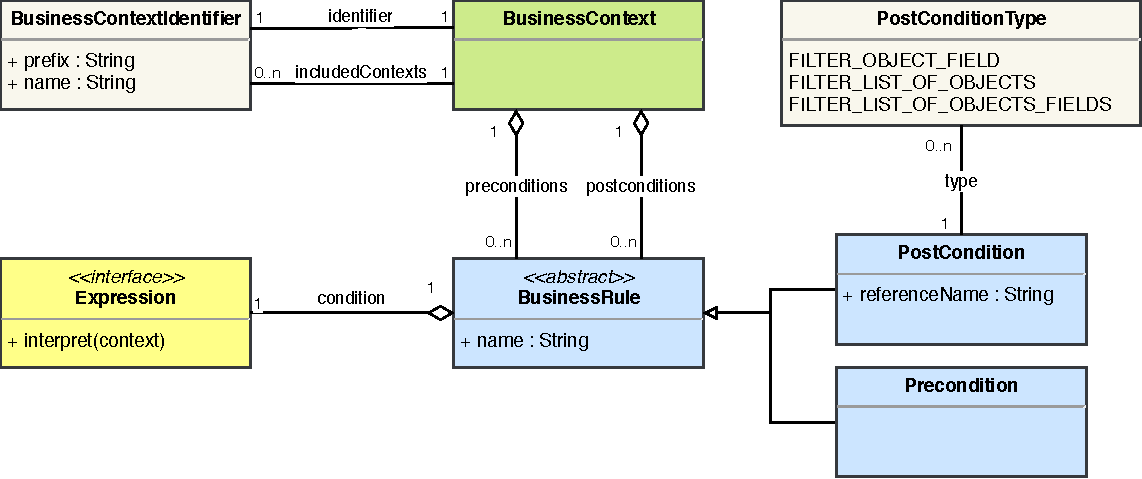
\includegraphics[keepaspectratio=true, width=\linewidth]{figures/business-context-metamodel.pdf}
    \caption{Diagram tř\'{\i}d metamodelu byznysového kontextu}
    \label{fig:business-context-metamodel}
\end{figure} % TODO: popsat

\section{Expression}

\section{Registr byznys kontextů}

\begin{figure}
    \centering
    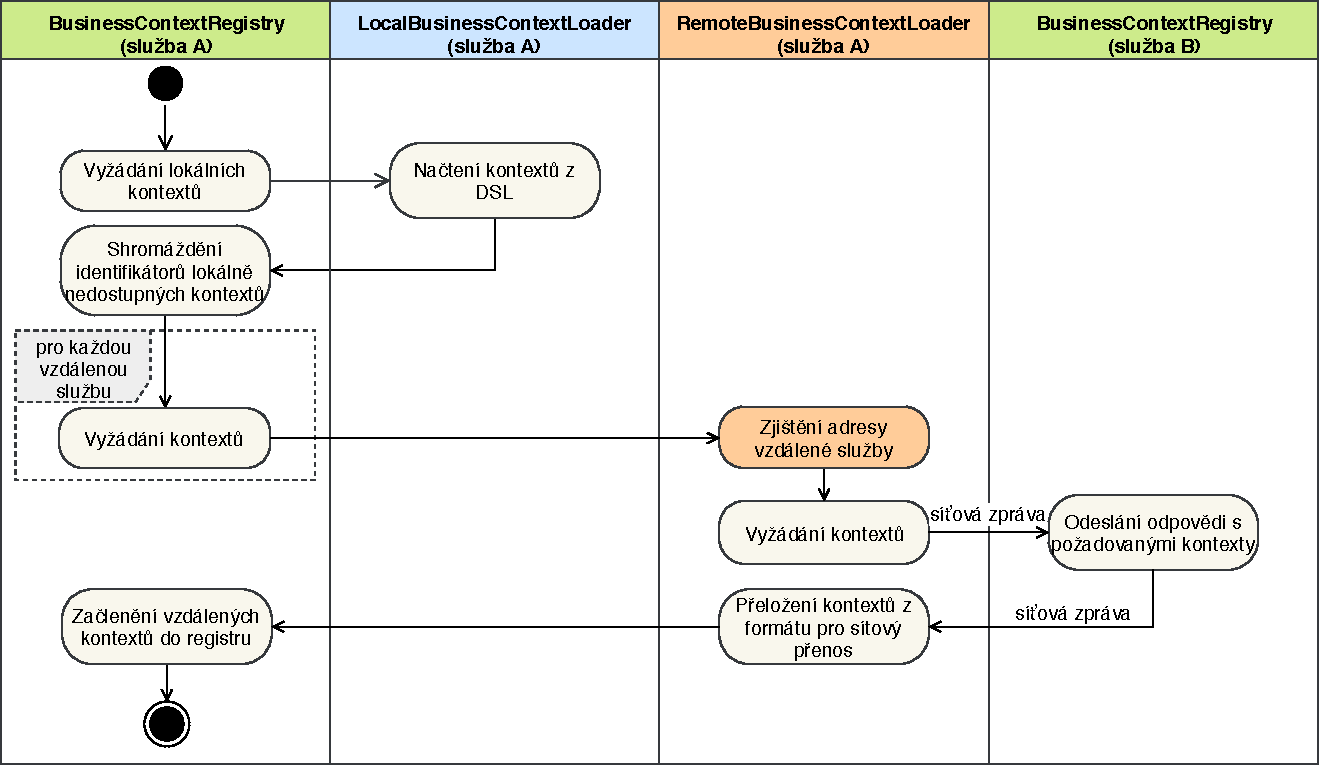
\includegraphics[keepaspectratio=true, width=0.8\linewidth]{figures/business-context-loading.pdf}
    \caption{Diagram procesu inicializace byznysov\'ych kontextů}
    \label{fig:business-context-loading}
\end{figure} % TODO: popsat

\section{Byznys kontext weaver}

\begin{figure}
    \centering
    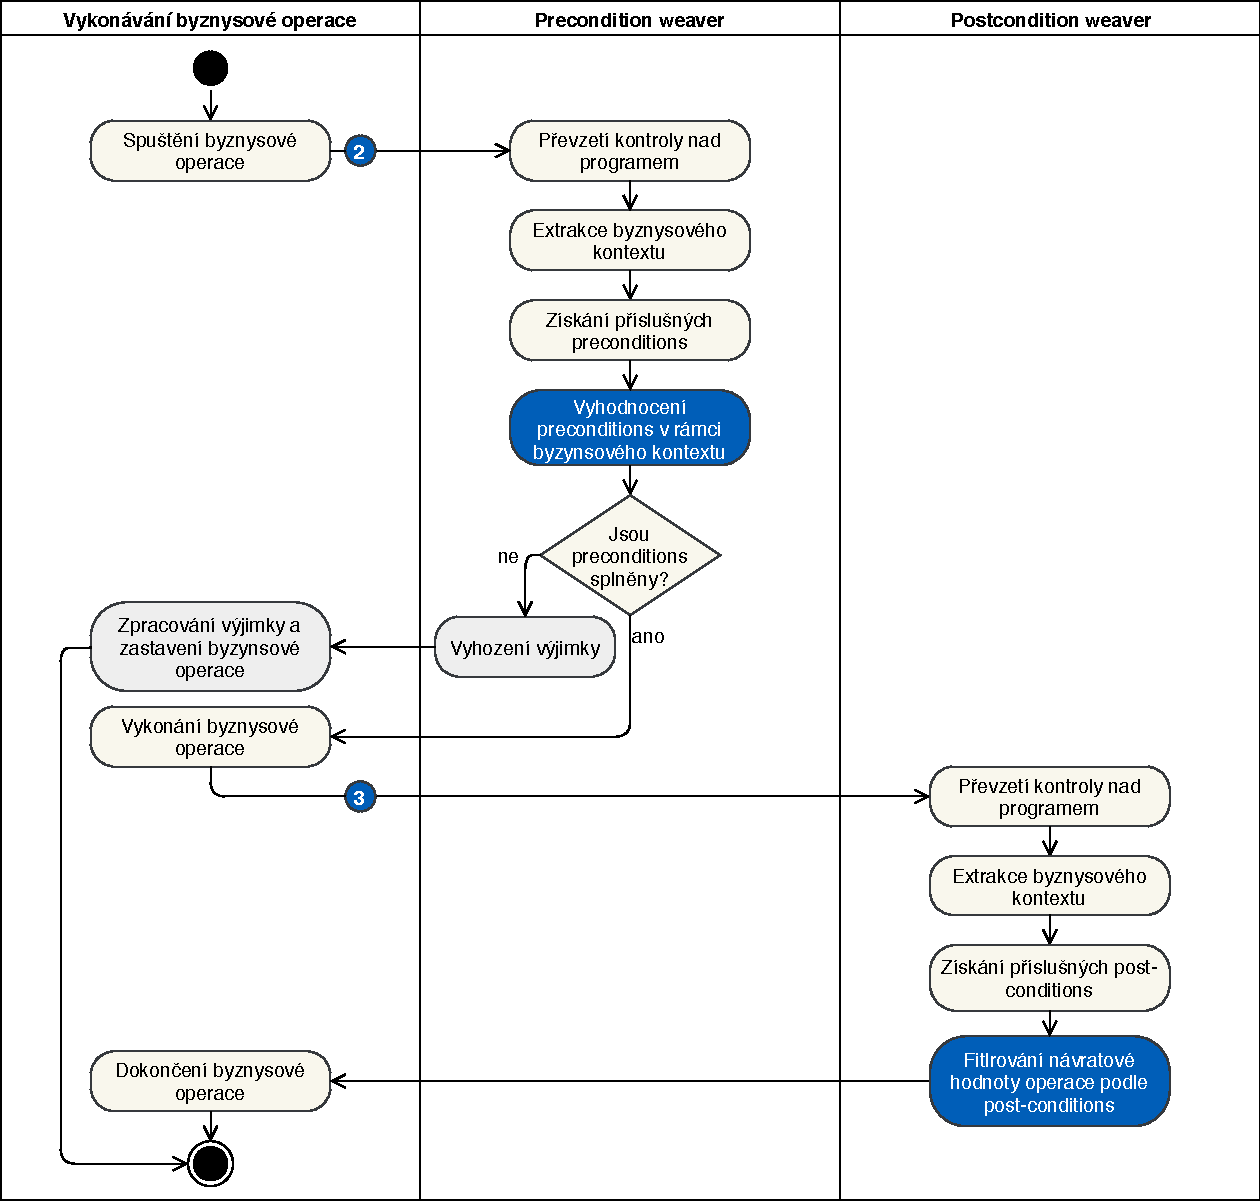
\includegraphics[keepaspectratio=true, width=0.8\linewidth]{figures/business-rules-weaver.pdf}
    \caption{Diagram aktivit weaverů byznysov\'ych pravidel}
    \label{fig:business-rules-weaver}
\end{figure} % TODO: popsat

\section{Centráln\'{\i} správa byznys kontextů}

Vzhledem k nutnosti centralizovat správu byznysových kontextů se nám
architektura \gls{P2P} představená v subsekci~\ref{sec:p2p} nehodí.
Při úpravě kotextů by totiž v systému mohly existovat staré i nové verze
byznysových pravidel, což je pro správnou funkci systém nepřijatelné.
Využijeme tedy architektury klient-server s více servery.
Byznysové kontexty budou podle svého prefixu rozděleny do skupin
a každou ze skupin bude spravovat jedna služba, která bude zároveň
držet jejich aktuální a jediný stav.

\begin{figure}
    \centering
    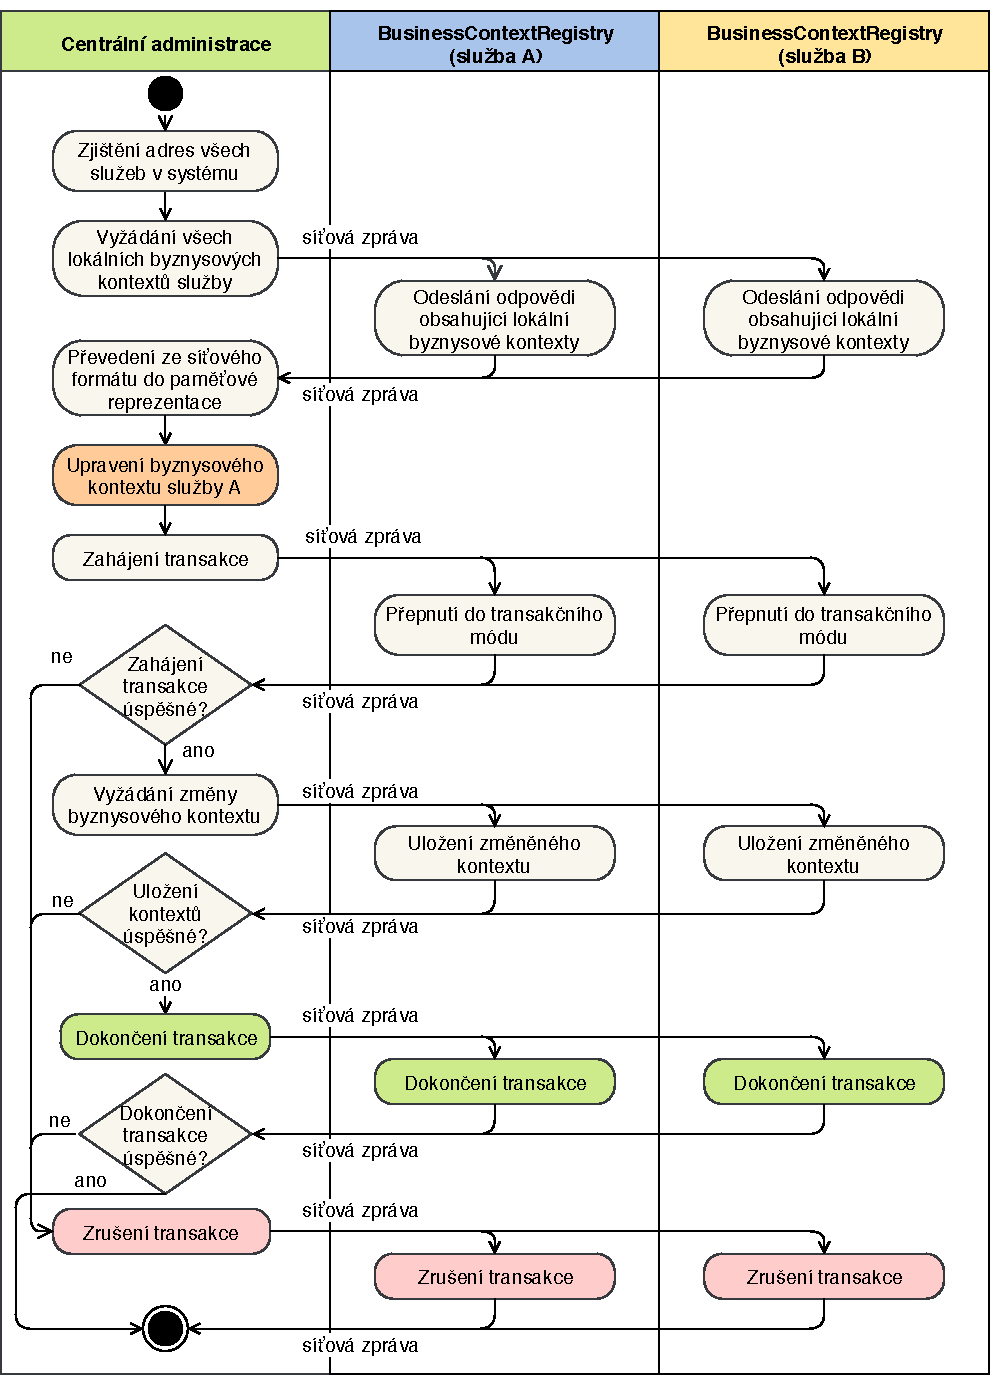
\includegraphics[keepaspectratio=true, width=0.8\linewidth]{figures/business-context-management.pdf}
    \caption{Diagram procesu centráln\'{\i} správy byznysov\'ych kontextů}
    \label{fig:business-context-management}
\end{figure} % TODO: popsat

\subsection{Uložen\'{\i} rozš\'{\i}řeného pravidla}

\goal{Diskutovat chaining vs. direct update}
% TODO: napiš mě

\section{Service discovery}

\goal{Popsat nezávislost na service discovery}
